\chapter{Examples I}
\label{examples_I}
In this chapter we will present some examples in order to reinforce and clarify various topics introduced in the previous chapters

\section{PI Cruise Controller}
In this example we will analyse the model of the closed loop cruise controller. This is shown in the image below


\begin{figure}[!htb]
\begin{center}
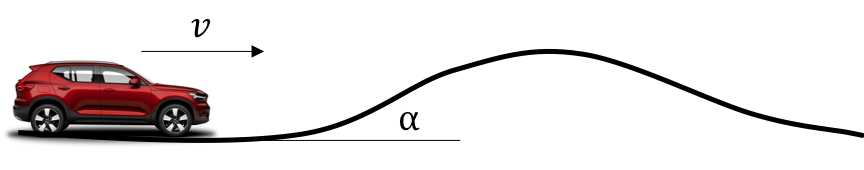
\includegraphics[scale=0.380]{img/model_based_eng/P1_1_2_1_ex_2.png}
\end{center}
\caption{Schematics of PI close loop cruise controller.}
\label{P1_1_2_1_ex_2}
\end{figure}

\begin{figure}[!htb]
\begin{center}
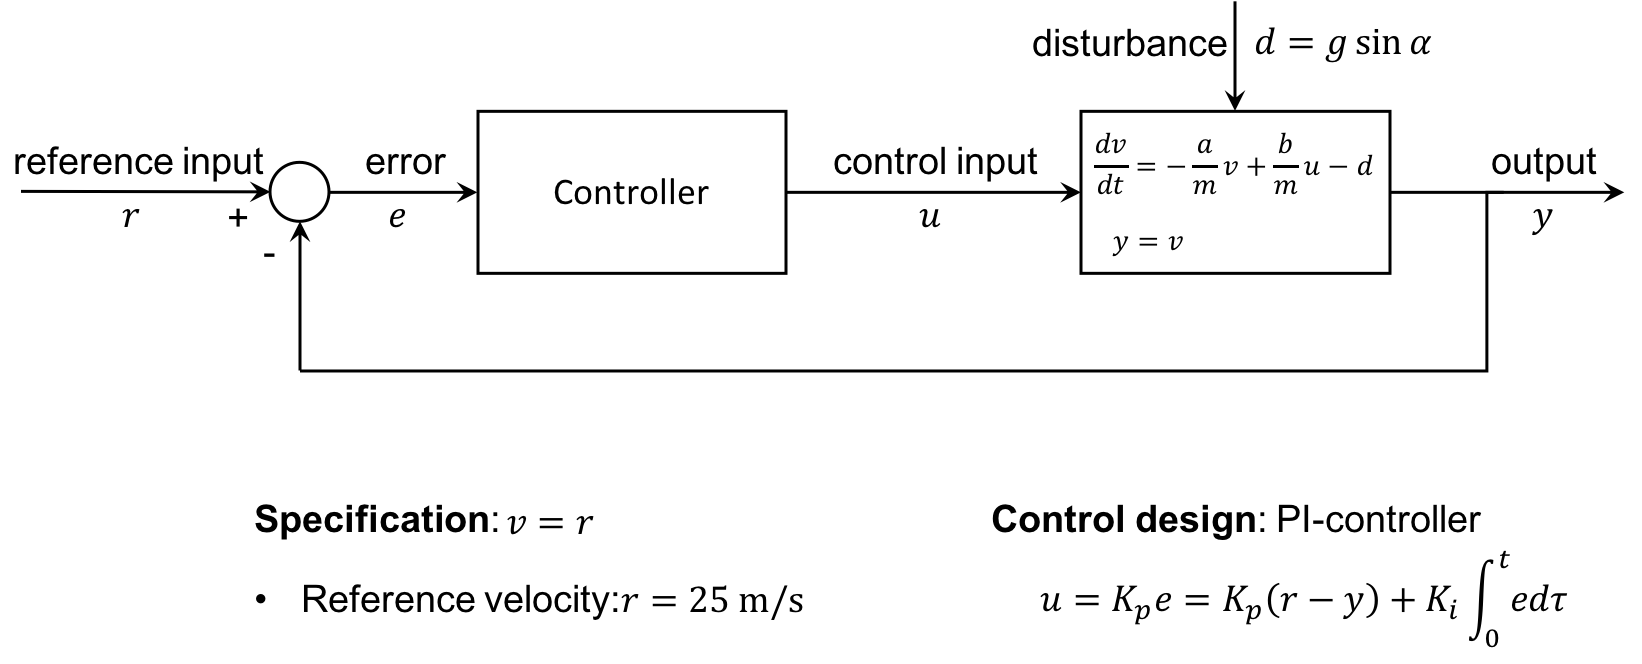
\includegraphics[scale=0.280]{img/model_based_eng/P2_1_2_1_ex_2_cruise.png}
\end{center}
\caption{Schematics of PI close loop cruise controller.}
\label{P2_1_2_1_ex_2_cruise}
\end{figure}


\subsection{Questions}

\textbf{Question 1:}

Which features are representative for a closed loop controller?

\begin{itemize}
\item A) Acts on deviation
\item B) No risk for instability
\item C) Risk for instability
\item D) Insensitive to measurement noise 
\end{itemize}

\textbf{Answer:}
A closed loop controller acts on the deviation from the reference signal in a measure-decide-act cycle. So 
option A is correct. Closed loop controllers are subject to instability problems; the closed loop dynamics can be shaped in such a way that the system might become unstable. So option C is also correct.


\textbf{Question 2:}

Which features are representative for an open loop controller?

\begin{itemize}
\item A) Acts on deviation
\item B) No risk for instability
\item C) Risk for instability
\item D) Insensitive to measurement noise 
\end{itemize}

\textbf{Answer:}
In an open loop controller all control actions are preprogrammed (otherwise we have no control). Thus, option A is correct. Option B is also correct provided that the system is also stable. In this case the open loop controller will also be stable. For an open loop controller no measurements are required, so no sensitivity towards measurements (VERIFY THIS). Thus, option D is also correct. 


\textbf{Question 3:}

Would you say that a driver is closed loop or open loop controller? 

\textbf{Answer:}
Since a driver typically aquires feedback via his/her senses and acts accordingly in order to adapt to the measured feedback, we can say that a driver is a closed loop controller.




